In general, PEFT methods can be divided into five main categories \cite{xu2023parameterefficient}:
\begin{enumerate}
    \item \textbf{additive fine-tuning}: these methods introduce new extra trainable parameters for task-specific fine-tuning. One can further divide into the following subcategories:
    \begin{enumerate}
        \item \textbf{Adapter-based Fine-tuning}: an adapter module is incorporated into the transformer, allowing for fine-tuning without modifying the pretrained parameters 
        \item \textbf{Soft Prompt-based Fine-tuning}: trainable continuous vectors, known as soft prompts, are inserted into the input or hidden state of the model. Unlike manually designed hard prompts, soft prompts are generated by searching for prompts in a discrete token space based on task-specific training data 
        \item \textbf{Others} 
    \end{enumerate}
    \item \textbf{Partial Fine-tuning}: aims at reducing the number of fine-tuned parameters by selecting a subset of pre-trained parameters that are critical to downstream tasks while discarding unimportant ones. We further differentiate between: 
    \begin{enumerate}
        \item \textbf{Bias Update}: only the bias term in the attention layer, feed-forward layer and layer normalization of the transformer is updated
        \item \textbf{Pretrained Weight Masking}: where the pretrained weights are masked using various pruning criterion
        \item \textbf{Delta Weight Masking}: delta weights are masked via pruning techniques and optimization approximation
    \end{enumerate}
    \item \textbf{Reparameterized Fine-tuning}: these methods utilize low-rank transformation to reduce the number of trainable parameters while allowing operating with high-dimensional matrices (e.g., pretrained weights)
    \begin{enumerate}
        \item \textbf{Low-rank Decomposition}: finds a lower rank matrix that captures the essential information of the original matrix while reducing computational complexity and memory usage by re-parameterizing the updated delta weight
        \item \textbf{LoRA Derivatives}: series of PEFT methods that are improved based on LoRA
    \end{enumerate}
    \item \textbf{Hybrid Fine-Tuning}: methods that aim to combine various PEFT approaches, such as adapter, prefix-tuning, and LoRA, to leverage the strengths of each method and mitigate their weaknesses
    \begin{enumerate}
        \item \textbf{Manual Combination}: mainly involves integrating the structure or features of one PEFT method into another PEFT method to enhance performance while achieving parameter efficiency
        \item \textbf{Automatic Combination}: explores how to configure PEFT methods like adapters, prefix-tuning, BitFit, and LoRA to different layers of the transformers automatically using various structure search and optimization approaches
    \end{enumerate}
    \item \textbf{Unified Fine-tuning}: lastly there are unified frameworks for fine-tuning, which streamlines the incorporation of diverse fine-tuning methods into a cohesive architecture, ensuring consistency and efficiency across the adaptation and optimization of models. Unlike hybrid fine-tuning methods, unified fine-tuning methods typically utilize a single PEFT method rather than a combination of various PEFT methods.
\end{enumerate}

% --------------BITFIT--------------

\noindent\todo{Eileen} \cite{zaken2022bitfit} BitFit Overview:
\begin{itemize}
    \item only the bias-terms of the model (or a subset of them) are being modified
    \item  freezing most of the network and fine-tuning only the bias-terms is surprisingly effective
    \item Three key properties
    \begin{enumerate}
        \item match the results of fully fine-tuned model
        \item enable tasks to arrive in a stream, this way it does not require simultaneous access to all datasets
        \item  fine-tune only a small portion of the model’s parameters
    \end{enumerate}
    \item trains less than 0.1\% of the total number of parameters
    \item Bitfit achieves transfer learning performance which is comparable (and sometimes better!) than fine-tuning of the entire network
\end{itemize}


% --------------LORA--------------

\textbf{Low Rank Adaptation (LoRA)} \cite{hu2021lora} is another PEFT method for fine tuning LLMs. Main principle behind LoRA is fixing the weights of the original model and then injecting trainable low rank decomposition matrix into the current LLM architecture. 

\begin{enumerate}
    \item \textbf{Architecture of the LoRA}

    Architecture of model is modified in following way. The original weights $W_{0}$ are fixed and additional trainable weights $\Delta W$ are introduced. $\Delta W$ can be decomposed to $BA$, where rank of both matrices $B$ and $A$ is much smaller than rank of the original $W_{0}$. Resulting weights are constructed as composition $W_{0} + \Delta W = W_{0} + BA$. This way much lower number of parameters is needed to be trained. Graphical depiction can be seen in Figure ~\ref{fig:LoRA}.

    \begin{figure}[h!]
        \centering
        {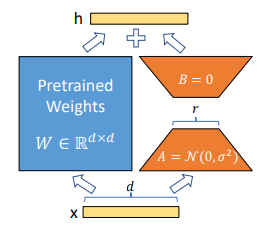
\includegraphics[scale=0.9]{imgs/LoRA.png}}
        \caption{schematic architecture of LoRa \cite{hu2021lora}}
        \label{fig:LoRA}
    \end{figure}
    
    \item \textbf{Empirical results}
    
    It turns out that LoRA performs similarly or even outperforms other methods compared in the paper, while having comparable or lower number of trainable parameters.
    For example comparing full finetuning of GPT-3 model with LoRA finetuning of the same model, the number of trainable parameters was reduced 10000 times and GPU memory requirement was reduced 3 times.
    
    Authors of the paper also noted that surprisingly low rank (as low as 1) is already yielding good results.
    
    \item \textbf{LoRA benefits}
    
    \begin{itemize}
        \item having relatively small amount of parameters to train
        \item not introducing additional latency, unlike e.g. adapter methods
        \item being able to deploy several specialized models at once, as LoRA reduces memory and computational footprint. LoRA does this by having several trained decomposition matrices for each specialized task while keeping the weights for the base model fixed.
    \end{itemize}
\end{enumerate}


% --------------PROMPT TUNING--------------

\textbf{The power of Scale for Parameter-Efficient Prompt Tunning}\cite{lester2021power} presents prompt tuning as an effective mechanism for conditioning frozen language models to perform specific tasks. The paper shows that prompt tuned T5-XXL model outperforms GPT-3 175B in SuperGLUE benchmark, despite having 16 times less parameters.


General overview:

\begin{itemize}
    \item definition of prompt tuning in the context of T5 fine tuning
    \item propose three options for initialization of prompt initialization and try different prompt lengths
    \item propose three methods for unlearning span corruption
    \item describe the results for different parameters
\end{itemize}

\begin{enumerate}
    \item \textbf{Prompt Tuning}
    
    Instead of modeling classification as the probability $Pr(y|X)$, it is modeled as $Pr(Y|X)$, where y is a single class label, Y is a sequence of tokens that represent a class label and X is a series of tokens. In T5 models in particular it is modeled as $Pr_\theta(Y|X)$
    When using prompt tuning the we use a $Pr_{\theta;\theta_p}(Y|[P;X])$ where P are prompt tokens. Models are trained to maximize the probability of Y, but only prompt parameters are updated.
    \begin{enumerate}
        \item \textbf{Design Decisions:} there are many ways of initializing the prompt representations. One possibility is training from scratch using random initialization. Better option is to initialize each prompt token to an embedding from models vocabulary. For classification tasks prompts could be initialized as embeddings that enumerate the output classes.
        \item \textbf{Unlearning Span Corruption:} span corruption could be a major problem of T5 model, so the paper describes experiments with three settings. "Span Corruption" uses pre-trained T5 as a frozen model. "Span Corruption + Sentinel" uses the same model but preappends setinels to all downstream targets. "LM Adaptation" continues with T5 self-supervised training for small number of additional steps, given a natural text prefix as input. LM adaptation transforms T5 into model more like GPT-3.
    \end{enumerate}
    \item  \textbf{Results}
    
    Frozen models ar built on top of pre-trained T5 checkpoints. The preformance is measured no SuperGLUE benchmark, each of the prompts is trained on a single SuperGLUE task. Prompts are tranied for 30000 steps using cross-entropy loss with a constant learning rate  of 0.3 and batch size of 32.
    \begin{enumerate}
        \item \textbf{Closing th Gap:} Prompt tuning becomes more competitive with model tuning as scale increases. When comparing with GPT-3 few shot preformance on SuperGLUE it is shown that T5-Small outperforms GPT-3 XL that is over 16 times larger.
        \item \textbf{Abation Study:}
        \begin{enumerate}
            \item Prompt lengths of sizes \{1, 5, 20, 100, 150\} were used, values above 20 produced only marginal increases
            \item Prompt initialization: for random initialization they sample uniformly from range [-0.5, 0.5]. For initialization from sampled vocabulary they restrict to 5000 most common tokens in T5's vocabulary. For "class label" initialization they take embeddings for the string representations of each class in downstream task. 
            \item Pre-training objective. The "span corruption" objective is not well suited for training frozen models and adding sentinels has little benefit. LM adaptation adds value across all model sizes.
        \end{enumerate}
    \end{enumerate}
\end{enumerate}